\section{Introduction}

\begin{figure}[t!]
    \centering
    \includegraphics[width=0.9\linewidth]{VITA-E//pic/vita-e-demo.png}
    \caption{VITA-E is capable of handling a variety of complex interactive scenarios, including nearly real-time concurrency and interruption. Please see our demo video in the supplementary material.}
    % at this \textbf{\href{https://youtu.be/jplQ0R50kfU}{YouTube link}.}}
    \label{fig:demo}
    \vspace{-2em}
\end{figure}

\begin{figure}[t!]
    \centering
    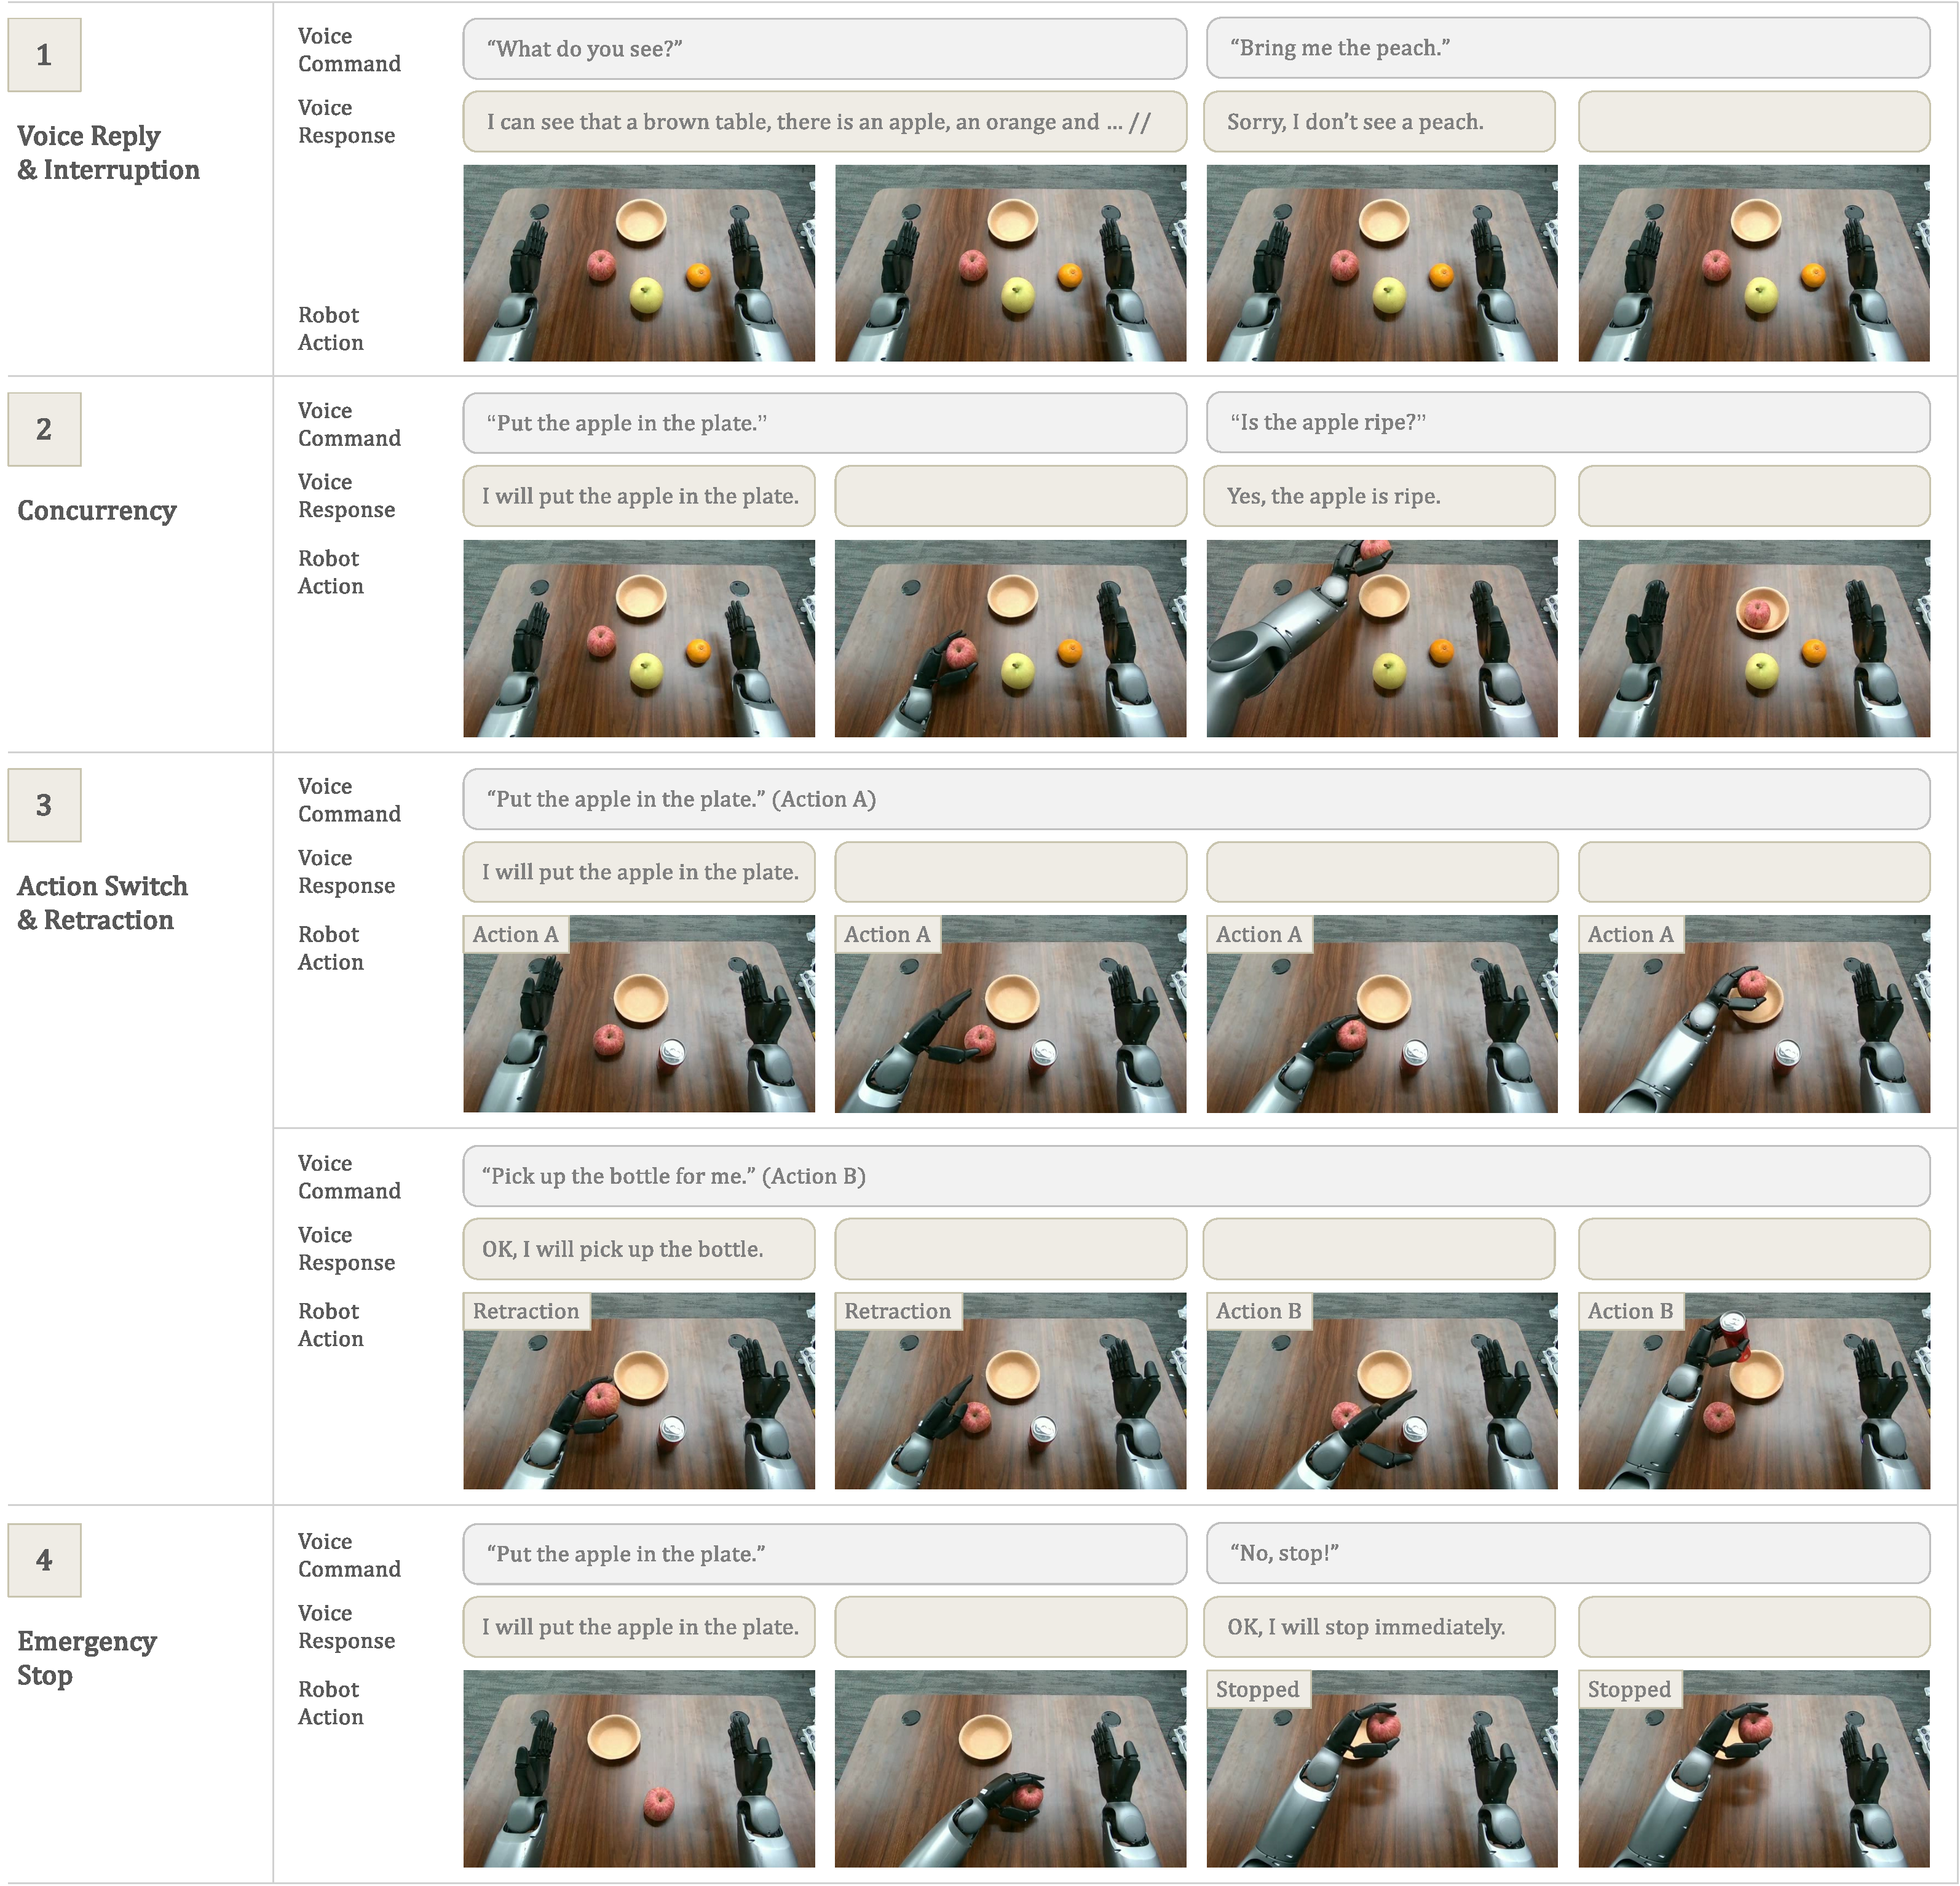
\includegraphics[width=\linewidth]{VITA-E//pic/demo.pdf}
    \caption{VITA-E's responses and actions in various interactive scenarios and instructions.}
    \label{fig:scenarios}
    \vspace{-2em}
\end{figure}

Humans naturally orchestrate complex interactions through the simultaneous integration of sight, sound, speech, and action, while fluidly adapting to and shifting between tasks. Achieving this level of seamless multimodal coordination is the defining aspiration for our ideal general-purpose robot. Thanks to advances in Vision-Language Models (VLMs)~\citep{qwenvl, internvl3, paligemma, gpt4}, the field of robotic control has rapidly evolved from task-specific imitation learning~\citep{act, ibc, rt1} towards more general-purpose multi-task action generation~\citep{rt2, openvla, octo} and open-ended instruction following~\citep{hirobot, gr00t, thinkact, ecot}, bringing us closer to this goal. However, the predominant focus of the field has been on improving the success rate of specific, static tasks, often overlooking a critical dimension of autonomy: the ability to engage in continuous, natural, and dynamic collaboration with a human user in complex scenarios~\citep{interactionhumanrobot, interactiverobots}. An ideal robotic assistant should not be a silent executor of commands but a collaborative partner, which encompasses maintaining continuous visual perception, processing auditory inputs, generating verbal responses, and executing physical actions in parallel (e.g., answering, ``Is the bookshelf tidied up?'' while organizing a room) and dynamically adapting to new directives that reflect a changing environment (e.g., ``Don't clean the bedroom yet---the baby is sleeping.''). Such concurrent multitasking and dynamic response is fundamental to enabling natural human-robot collaboration.

Although some work has begun to address complex instructions and human feedback~\citep{hirobot, saycan, yay, switchvla}, existing systems are fundamentally constrained by a rigid and static interaction paradigm. This paradigm imposes three critical limitations that prevent flexible human-robot collaboration: 1) \textbf{Lack of Concurrency:} Systems typically cannot perceive their environment and user while simultaneously responding verbally and acting physically, limiting their efficiency and ability to multitask in a human-like manner. 2) \textbf{Uninterruptibility:} Once engaged in an action or verbal response, the robot becomes locked into that behavior and cannot be interrupted by urgent user needs, forcing unnatural pauses and preventing fluid adaptation to changing priorities. 3) \textbf{Interaction inflexibility:} Together, these constraints create a stilted, unresponsive experience where the robot feels slow and unnatural to interact with, fundamentally preventing it from achieving the desired state of seeing, hearing, speaking, and acting simultaneously in real-time collaboration with humans.

To break through this paradigm bottleneck, we design and implement VITA-E, a system architected specifically for natural human-robot interaction. As shown in Figure~\ref{fig:demo} and Figure~\ref{fig:scenarios}, VITA-E is capable of handling these complex interactive scenarios. Inspired by the cooperative mechanism of the human brain's hemispheres and the interruptible model VITA~\citep{vita}, our framework features a novel dual-model interaction core. In this design, one model instance acts as the ``executing hemisphere,'' focused on the current task, while the other acts as a ``listening hemisphere'', ready to process new user requests. This parallel architecture fundamentally overcomes the limitations of sequential execution, achieving the capability of ``seeing, hearing, speaking, and acting simultaneously'' for a VLA system.

Our primary contributions are as follows:
\begin{itemize}
    \item \textbf{A Dual-Model Architecture for Concurrent Interaction:} We introduce a novel parallel processing framework where two VLA instances work in concert. One acts as an active model for the current task, while the other serves as a standby model, enabling behavioral concurrency, as well as the instant interruption of any ongoing task or response.
    \item \textbf{A Special Token-Based Control Flow:} We design a set of special tokens (e.g., \texttt{[ACT]}, \texttt{[HALT]}) that are generated by the VLM itself to directly drive the system's state transitions. This ``model-as-controller'' paradigm creates an elegantly tight coupling between action and system behavior.
    \item \textbf{A Methodology for Training Interactive VLAs:} We introduce a data curation and fine-tuning strategy to teach a VLM to generate system-level control tokens. Our methodology is implemented upon a mainstream VLM + Diffusion Action Expert architecture, demonstrating its compatibility with a wide range of state-of-the-art dual-system models.
\end{itemize}
